\documentclass[11pt]{article}

\pdfpagewidth 8.5in
\pdfpageheight 11in

\setlength\topmargin{0in}
\setlength\headheight{0in}
\setlength\headsep{0.4in}
\setlength\textheight{8in}
\setlength\textwidth{6in}
\setlength\oddsidemargin{0in}
\setlength\evensidemargin{0in}
\setlength\parindent{0.25in}
\setlength\parskip{0.1in} 
 
\usepackage{amssymb}
\usepackage{amsfonts}
\usepackage{amsmath}
\usepackage{mathtools}
\usepackage{amsthm}

\usepackage{fancyhdr}

\usepackage{enumerate}

      \theoremstyle{plain}
      \newtheorem{theorem}{Theorem}
      \newtheorem{lemma}[theorem]{Lemma}
      \newtheorem{corollary}[theorem]{Corollary}
      \newtheorem{proposition}[theorem]{Proposition}
      \newtheorem{conjecture}[theorem]{Conjecture}
      \newtheorem{question}[theorem]{Question}
      
      \theoremstyle{definition}
      \newtheorem{definition}[theorem]{Definition}
      \newtheorem{example}[theorem]{Example}
      \newtheorem{game}[theorem]{Game}
      
      \theoremstyle{remark}
      \newtheorem{remark}[theorem]{Remark}



\pagestyle{fancy}
\renewcommand{\headrulewidth}{0.5pt}
\renewcommand{\footrulewidth}{0pt}
\lfoot{\small \jobname.tex -- Updated on \today}
\chead{\small http://github.com/StevenClontz/Research}
\rfoot{\thepage}
\cfoot{}


% Strategy uparrow shortcuts
\newcommand{\win}{\uparrow}
\newcommand{\prewin}{\uparrow_{\text{pre}}}
\newcommand{\markwin}{\uparrow_{\text{mark}}}
\newcommand{\tactwin}{\uparrow_{\text{tact}}}
\newcommand{\ktactwin}[1]{\uparrow_{#1\text{-tact}}}
\newcommand{\kmarkwin}[1]{\uparrow_{#1\text{-mark}}}
\newcommand{\codewin}{\uparrow_{\text{code}}}
\newcommand{\limitwin}{\uparrow_{\text{limit}}}

\newcommand{\oneptcomp}[1]{#1^*}
\newcommand{\oneptlind}[1]{#1^\dagger}

\newcommand{\congame}[2]{Con_{O,P}(#1,#2)}
\newcommand{\clusgame}[2]{Clus_{O,P}(#1,#2)}

\newcommand{\lfkpgame}[1]{LF_{K,P}(#1)}
\newcommand{\lfklgame}[1]{LF_{K,L}(#1)}

\newcommand{\pfgame}[1]{PF_{F,C}(#1)}

\newcommand{\mengame}[1]{Cov_{C,F}(#1)}
\newcommand{\rothgame}[1]{Cov_{C,S}(#1)}
\newcommand{\altrothgame}[1]{Cov_{P,O}(#1)}

\newcommand{\fillgame}[1]{Fill^{\subseteq}_{M,N}(#1)}
\newcommand{\sfillgame}[1]{Fill^{\subsetneq}_{M,N}(#1)}

\newcommand{\kfillgame}[1]{Fill^{\subseteq}_{C,F}(#1)}
\newcommand{\ksfillgame}[1]{Fill^{\subsetneq}_{C,F}(#1)}

\newcommand{\sigmaprodr}[1]{\Sigma\mathbb{R}^{#1}}
\newcommand{\sigmaprodtwo}[1]{\Sigma2^{#1}}

\newcommand{\concat}{^\frown}
\newcommand{\rest}{\restriction}

\newcommand{\cl}[1]{\overline{#1}}

\newcommand{\pow}[1]{\mc{P}(#1)}

\newcommand{\<}{\langle}
\renewcommand{\>}{\rangle}

\newcommand{\mc}[1]{\mathcal{#1}}

\newcommand{\Lim}{\mathrm{Lim}}
\newcommand{\Suc}{\mathrm{Suc}}

\newcommand{\ds}{\displaystyle}

\newcommand{\rank}{\textrm{rank}}

\newcommand{\scish}{$\sigma$-compactish }



\begin{document}

\centerline{\bf An Example of Gruenhage's Compact-Point Game for which $K$ has }
\centerline{\bf a winning strategy, but no winning $k$-Markov strategy}

We construct a ZFC example given by Gary Gruenhage, inpsired by a ZFC+$\lnot$SH example due to Stephen Watson \cite{Watson}. We require a result of Gruenhage and Michael \cite{Michael}:

\begin{theorem}\label{michael}
Let $X$ be a meta-Lindel\"of, locally Lindel\"of regular space, and let $\mc{B}$ be a base for $X$. Then $X$ has a cover $\mc{B}'\subseteq\mc{B}$ such that $\{\close{B}:B\in\mc{B}'\}$ is point-countable.
\end{theorem}

\begin{theorem}\label{basic_x}
There exists a compact, zero-dimensional topological space $X$ and an uncountable subspace $C\subseteq 2^\omega$ of the Cantor Set, such that $X$ has a point-countable cover $\mc{U} = \{U_c : c \in C\}$ of clopen sets which is not $\sigma$-point-finite (the union of countably-many point-finite collections).
\end{theorem}

\begin{proof}
Take a zero-dimensional Corson compact $Y$ of weight $2^\omega$, which is not Eberlein compact. (See Todercevic \cite{Todercevic} for an example.) It follows by \cite{G1} that $Y^2$ is hereditarily metaLindel\"of, but not hereditarily $\sigma$-metacompact. Note $X=Y^2\setminus \Delta$ is an open non-$\sigma$-metacompact subspace of $Y^2$, and thus locally compact, and let $\mc{V}$ be an open cover of $X$ such that no $\sigma$-point-finite open refinement exists.

Let $\mc{B}$ be a clopen base for $X$ of cardinality $2^\omega$ which is a refinement of $\mc{V}$.  Then as $X$ is metaLindel\"of, locally Lindel\"of, and regular, by Thm \ref{michael}, let $\mc{U}\subseteq \mc{B}$ be a point-countable clopen refinement of $\mc{V}$ of cardinality $\leq 2^\omega$, which cannot be $\sigma$-point-finite (and is thus uncountable).
\end{proof}

\begin{definition}
Using the $X$ from Theorem \ref{basic_x}, let \[\mathbb{X} = (X \times 2^{<\omega}) \cup 2^\omega\] compose a topological sum of $2^{<\omega}$ copies of $X$ along with a discrete copy of a subspace $C \subseteq 2^\omega$ of the Cantor Set, and add open (in fact, compact) neighborhoods of the form: 
  \[
    B_c = c \cup (U_c \times \{c\rest n : n < \omega\})
  \]
as seen in Figure \ref{fig:cantor_tree}.
\end{definition}

\begin{figure}[p]
  \centering
  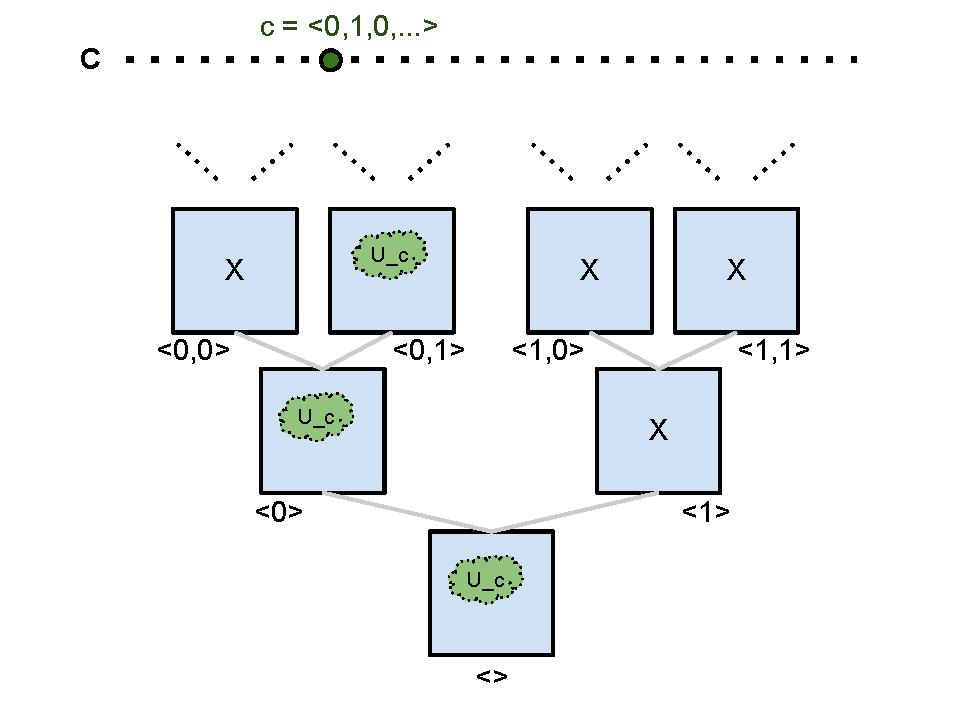
\includegraphics[width=6in]{cantor_tree_open.pdf}
  \caption{The Cantor Tree space $\mathbb{X}$}
  \label{fig:cantor_tree}
\end{figure}

\begin{definition}
Let $S\in[C]^{<\omega}$ and $m<\omega$. Define 
  \[
    K_S = \bigcup_{c \in S} B_c
  \] 
  \[ 
    A = \{z^\frown \<1\> : z \in 1^{<\omega}\}
  \] 
  \[ 
    K^*_S = K_S \setminus (X \times A)
  \] 
  \[
    L_m = X \times 2^{<m}
  \] 
and observe that every compact set is dominated by the compact set $K^*_S \cup L_m$ for some $S,m$.

Intuitively, $K^*_S$ collects the branches of $U_c$ converging up to each $c \in S$ while avoiding the copy of $X$ for each $s$ in an antichain $A$, and $L_m$ collects the copies of $X$ with $|s| < m$ at the base of the tree. (See Figure \ref{fig:cantor_tree_compact})
\end{definition}

\begin{figure}[p]
  \centering
  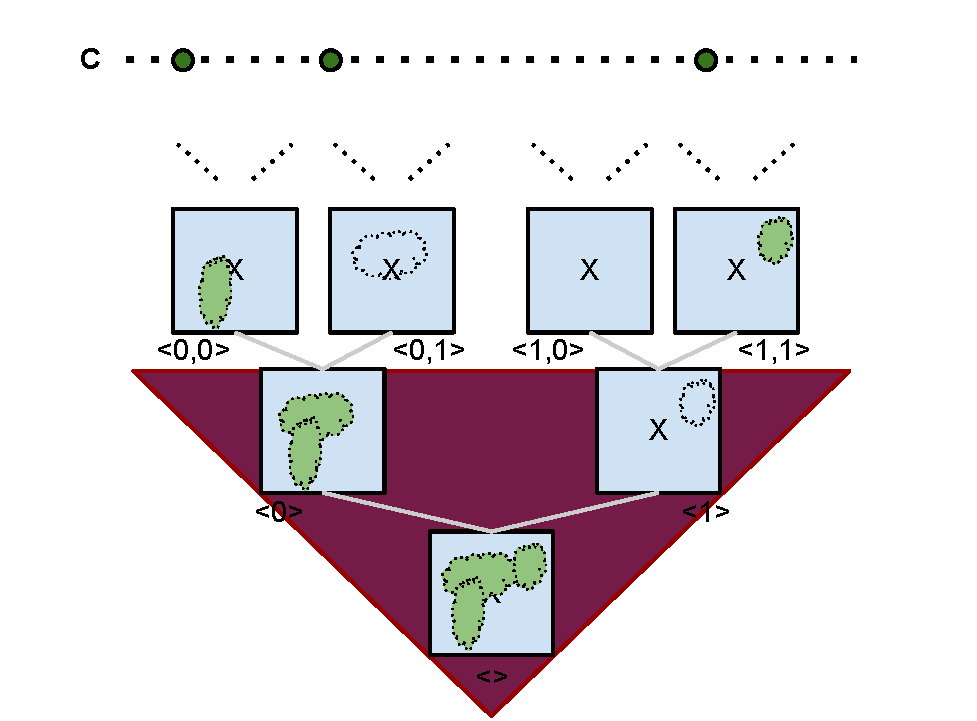
\includegraphics[width=6in]{cantor_tree_compact.pdf}
  \caption{$K^*_S$ and $L_m$}
  \label{fig:cantor_tree_compact}
\end{figure}

\begin{definition}
$\lfkpgame{\mathbb{X}}$ is a topological game consisting of players $K$ and $P$. During each round, $K$ chooses a compact subset of $\mathbb{X}$, and $P$ chooses a point outside of any compact set previously played by $K$. $K$ wins the game if the set of points chosen by $P$ throughout all rounds of the game are locally finite in the space.
\end{definition}

\begin{definition}
We say $I \win G$ if Player $I$ has a winning strategy in the game $G$.

We say $I \tactwin G$ (resp. $I \ktactwin{k} G$) if Player $I$ has a winning tactical (resp. $k$-tactical) strategy in the game $G$, a strategy depending on only the ($k$) most recent move(s) of the opponent.

We say $I \markwin G$ (resp. $I \kmarkwin{k} G$) if Player $I$ has a winning Markov (resp. $k$-Markov) strategy in the game $G$, a strategy depending on only the ($k$) most recent move(s) of the opponent and the current round number.
\end{definition}

\begin{proposition}
Without loss of generality, we may assume $P$ always plays points in $X \times 2^{<\omega}$ throughout $\lfkpgame{\mathbb{X}}$.
\end{proposition}

\begin{proposition}
$K \win \lfkpgame{\mathbb{X}}$
\end{proposition}

\begin{proof}
Let $x\in X$. $C^x = \{c \in C : x \in U_c\}$ is a countable collection by the point-countability of $\mc{U}$, so label its elements as $\{c^x_n: n<\omega\}$.

$K$ may use the strategy 
  \[
    \sigma(\<x_0,s_0\>,\dots,\<x_{n-1},s_{n-1}\>) = 
    \bigcup_{i < n} K_{\{c^{x_i}_0,\dots,c^{x_i}_{n-1}\}} \cup L_{|s_i|+1}
  \]

This is a winning strategy because each move $\<x_i,s_i\>$ by $P$ cannot be a part of a subsequence of the play converging to any $c^{x_i}_n$, since $K_{\{c^{x_i}_0,\dots,c^{x_i}_n\}} \supseteq B_{c^{x_i}_n}$ was forbidden during round $n$.
\end{proof}

\begin{theorem}
$K\not\tactwin\lfkpgame{\mathbb{X}}$.
\end{theorem}

\begin{proof}
This is actually a corollary of Gruenhage's theorem in \cite{G2}: $\mathbb{X}$ is locally compact (each point is either in some $X$ or in some $B_c$) but not metacompact (any cover of $C$ necessarily will have infinite overlap at some $X \times \{s\}$). However, we proceed with a direct game-theoretic proof.

Suppose that $\sigma(\<x,s\>)$ was a winning tactical strategy for $K$ and define the compact set 
  \[
    \sigma'(x,n) = \bigcup_{|s|\leq n} \sigma(\<x,s\>)
  \]

There exists some $f: C \to \omega$ such that for all $x\in U_c$, $\sigma'(x,f(c))$ covers some $B_c \setminus L_m$. (If not, $P$ counters by simply always playing in $B_c \setminus L_m$.)

Recall that $\mc{U}$ is not the union of the countably-many point-finite collections, and 
  \[
    \mc{U} = \bigcup_{n<\omega} \{U_c : f(c) = n\}
  \]
so we may choose $n$ where $\mc{U}_n = \{U_c : f(c) = n\}$ is not point-finite. Fix $x$ so that $x$ belongs to each of $\{U_{c_0},U_{c_1},\dots\} \subseteq \mc{U}_n$.

For each $c_i$, $\sigma'(x,f(c_i))=\sigma'(x,n)$ covers $c_i$. Thus $\sigma'(x,n) \supseteq \{c_0,c_1,\dots\}$ is a compact set covering a closed discrete subset, a contradiction.
\end{proof}

\begin{theorem}
$K\not\ktactwin{2}\lfkpgame{\mathbb{X}}$.
\end{theorem}

\begin{proof}
Suppose $\sigma(\<x,s\>,\<y,t\>)$ was a winning 2-tactical strategy. Without loss of generality we assume it ignores order. We may define $S(x,y,n)\in [C]^{<\omega}$ (increasing on $n$) and $n<m(x,y,n)<\omega$ such that for each $(x,y)$,
  \[
    \bigcup_{s,t \in 2^{\leq n}} \sigma(\<x,s\>,\<y,t\>) \subseteq 
    K^*_{S(x,y,n)} \cup L_{m(x,y,n)}
  \]
and so we assume
  \[
    \sigma(\<x,s\>,\<y,t\>) =
    K^*_{S(x,y,\max(|s|,|t|))} \cup L_{m(x,y,\max(|s|,|t|))}
  \]

Select an arbitrary point $x' \in X$. We define a tactical strategy 
  \[
  \tau(x,s) = 
  K^*_{S(x,x',m(x,x',|s|)+1)} \cup L_{m(x,x',m(x,x',|s|)+1)}
  \]
We complete the proof by showing $\tau$ is a winning tactical strategy (a contradiction).

Suppose
\[
\<x_0, s_0\>, \<x_1, s_1\>, \<x_2, s_2\>, \dots
\]
successfully countered $\tau$ by clustering at $c\in C$ (the strategy trivially prevents clustering elsewhere). Let $z_n = \<0,\dots,0\>$ with $n$ zeros. We claim
\[
\<x_0, s_0\>, \<x', {z_{m(x_0,x',|s_0|)}}^\frown\<1\>\>, \<x_1, s_1\>, \<x', {z_{m(x_1,x',|s_1|)}}^\frown\<1\>\>,  \<x_2, s_2\>, \<x', {z_{m(x_2,x',|s_2|)}}^\frown\<1\>\>, \dots
\]
is a successful counter to $\sigma$.

We will need the fact that, as $\<x_{i+1},s_{i+1}\>$ was legal against $\tau$:
  \[
    |s_i| <
    m(x_i,x',|s_i|)+1 =
    |{z_{m(x_i,x',|s_i|)}}^\frown\<1\>| 
  \]
  \[
    <
    m(x_i,x',m(x_i,x',|s_i|)+1) =
    m(x_i,x',|{z_{m(x_i,x',|s_i|)}}^\frown\<1\>|) \leq
    |s_{i+1}|
  \]

Note that $m(x,y,\max(|s|,|t|))$ is increasing throughout this play of the game versus $\sigma$:
  \[
    m(x_i,x',\max(|s_i|,|{z_{m(x_i,x',|s_i|)}}^\frown\<1\>|))
  \]
  \[
    =
    m(x_i,x',|{z_{m(x_i,x',|s_i|)}}^\frown\<1\>|)
  \]
  \[
    \leq
    |s_{i+1}| 
  \]
  \[
    <
    m(x_{i+1},x',|s_{i+1}|)
  \]
  \[
    =
    m(x_{i+1},x',\max(|s_{i+1}|,|{z_{m(x_i,x',|s_i|)}}^\frown\<1\>|))
  \]
  \[
    =
    |{z_{m(x_{i+1},x',|s_{i+1}|)}}|
  \]
  \[
    <
    |{z_{m(x_{i+1},x',|s_{i+1}|)}}^\frown\<1\>|
  \]
  \[
    <
    m(x_{i+1},x',|{z_{m(x_{i+1},x',|s_{i+1}|)}}^\frown\<1\>|)
  \]
  \[
    =
    m(x_{i+1},x',\max(|s_{i+1}|,|{z_{m(x_{i+1},x',|s_{i+1}|)}}^\frown\<1\>|))
  \]

We turn to showing that $\<x', {z_{m(x_{i+1},x',|s_{i+1}|)}}^\frown\<1\>\>$ is always a legal move. Since ${z_{m(x_{i+1},x',|s_{i+1}|)}}^\frown\<1\>$ is on the antichain avoided by any $K^*$, the problem is reduced to showing that this move isn't forbidden by
  \[
  L_{m(x_{i+1},x',\max(|s_{i+1}|,|{z_{m(x_i,x',|s_i|)}}^\frown\<1\>|))}
  \]
which we can see here:
  \[
    m(x_{i+1},x',\max(|s_{i+1}|,|{z_{m(x_i,x',|s_i|)}}^\frown\<1\>|)) =
    m(x_{i+1},x',|s_{i+1}|) <
    |{z_{m(x_{i+1},x',|s_{i+1}|)}}^\frown\<1\>|
  \]

We can conclude by showing that $\<x_{i+1},s_{i+1}\>$ is always a legal move. We can see it avoids 
  \[
  L_{m(x_{i},x',\max(|s_{i}|,|{z_{m(x_i,x',|s_i|)}}^\frown\<1\>|))}
  \]
since
  \[
    m(x_{i},x',\max(|s_{i}|,|{z_{m(x_i,x',|s_i|)}}^\frown\<1\>|)) =
    m(x_{i},x',|{z_{m(x_i,x',|s_i|)}}^\frown\<1\>|) \leq
    |s_{i+1}|
  \]

Since $\<x_{i+1},s_{i+1}\>$ was legal against $\tau$, for $h\leq i$ it avoided
  \[
    K^*_{S(x_h,x',m(x_h,x',|s_h|)+1)} = 
    K^*_{S(x_h,x',\max(|s_h|,|{z_{m(x_h,x',|s_h|)}}^\frown\<1\>|))}
  \]
and when $h<i$, we see it avoids:
  \[
    K^*_{S(x_{h+1},x',\max(|s_{h+1}|,|{z_{m(x_h,x',|s_h|)}}^\frown\<1\>|))} =
    K^*_{S(x_{h+1},x',|s_{h+1}|)}
  \]
  \[
    \subseteq
    K^*_{S(x_{h+1},x',m(x_{h+1},x',|s_{h+1}|)+1)}
  \]

This concludes the proof.
\end{proof}

\newpage

\begin{theorem}
$K\not\ktactwin{k}\lfkpgame{\mathbb{X}}$.
\end{theorem}

\begin{proof}
The proof proceeds in parallel to the proof of $K\not\ktactwin{2}\lfkpgame{\mathbb{X}}$, and in fact is just a generalization of said proof (at the cost of simplicity).

Suppose $\sigma(\<x_0,s_0\>,\dots,\<x_{k},s_{k}\>)$ was a winning $(k+1)$-tactical strategy. Without loss of generality we assume it ignores order. We may define $S(x_0,\dots,x_{k},n)\in [C]^{<\omega}$ (increasing on $n$) and $n<m(x_0,\dots,x_{k},n)<\omega$ such that for each $(x_0,\dots,x_{k})$,
  \[
    \bigcup_{s_0,\dots,s_k \in 2^{\leq n}} \sigma(\<x_0,s_0\>,\dots,\<x_{k},s_{k}\>) \subseteq 
    K^*_{S(x_0,\dots,x_{k},n)} \cup L_{m(x_0,\dots,x_{k},n)}
  \]
and so we assume
  \[
    \sigma(\<x_0,s_0\>,\dots,\<x_{k},s_{k}\>) =
    K^*_{S(x_0,\dots,x_{k},\max(|s_0|,\dots,|s_k|))} \cup L_{m(x_0,\dots,x_{k},\max(|s_0|,\dots,|s_k|))}
  \]

Select an arbitrary point $x' \in X$. Let $M^0(x,n)=m(x,x',\dots,x',n)$ and $M^{i+1}(x,n)=M^0(x,M^i(x,n)+1)$. We define a tactical strategy 
  \[
  \tau(x,s) = K^*_{S(x,x',\dots,x',M^{k-1}(x,|s|)+1)} \cup L_{m(x,x',\dots,x',M^{k-1}(x,|s|)+1)}
  \]
We complete the proof by showing $\tau$ is a winning tactical strategy (a contradiction).

Suppose
\[
\<x_0, s_0\>, \<x_1, s_1\>, \<x_2, s_2\>, \dots
\]
successfully countered $\tau$ by clustering at $c\in C$ (the strategy trivially prevents clustering elsewhere). Let $z_n = \<0,\dots,0\>$ with $n$ zeros. We claim
\[
  \<x_0, s_0\>, 
  \<x', {z_{M^0(x_0,|s_0|)}}^\frown\<1\>\>,
  \<x', {z_{M^1(x_0,|s_0|)}}^\frown\<1\>\>, 
  \dots, 
  \<x', {z_{M^{k-1}(x_0,|s_0|)}}^\frown\<1\>\>,
\]
\[
  \<x_1, s_1\>, 
  \<x', {z_{M^0(x_1,|s_1|)}}^\frown\<1\>\>, 
  \<x', {z_{M^1(x_1,|s_1|)}}^\frown\<1\>\>, 
  \dots, 
  \<x', {z_{M^{k-1}(x_1,|s_1|)}}^\frown\<1\>\>, 
  \dots
\]
is a successful counter to $\sigma$.

We will need the fact that, as $\<x_{i+1},s_{i+1}\>$ was legal against $\tau$:
  \[
    |s_i| <
    M^0(x_i,|s_i|)+1 =
    |{z_{M^0(x_i,|s_i|)}}^\frown\<1\>| <
    M^0(x_i,M^0(x_i,|s_i|)+1)+1 
  \]
  \[
    =
    M^1(x_i,|s_i|)+1 =
    |{z_{M^1(x_i,|s_i|)}}^\frown\<1\>| <
    \dots <
    |{z_{M^{k-1}(x_i,|s_i|)}}^\frown\<1\>| 
  \]
  \[
    =
    M^{k-1}(x_i,|s_i|) + 1 <
    m(x_i,x',\dots,x',M^{k-1}(x_i,|s_i|)+1) \leq
    |s_{i+1}|
  \]

Note that $m(x_0,\dots,x_{k},\max(|s_0|,\dots,|s_k|))$ is increasing throughout this play of the game versus $\sigma$:
  \[
    m(x_i,x',\dots,x',\max(|s_i|,|{z_{M^0(x_i,|s_i|)}}^\frown\<1\>|,\dots,|{z_{M^{k-1}(x_i,|s_i|)}}^\frown\<1\>|))
  \]
  \[
    =
    m(x_i,x',\dots,x',|{z_{M^{k-1}(x_i,|s_i|)}}^\frown\<1\>|)
  \]
  \[
    =
    m(x_i,x',\dots,x',M^{k-1}(x_i,|s_i|)+1)
  \]
  \[
    \leq
    |s_{i+1}| 
  \]
  \[
    <
    M^0(x_{i+1},|s_{i+1}|)
  \]
  \[
    =
    m(x_{i+1},x',\dots,x',|s_{i+1}|)
  \]
  \[
    =
    m(x_{i+1},x',\dots,x',\max(|s_{i+1}|,|{z_{M^0(x_i,|s_i|)}}^\frown\<1\>|,\dots,|{z_{M^{k-1}(x_i,|s_i|)}}^\frown\<1\>|))
  \]
  \[
    =
    |{z_{m(x_{i+1},x',\dots,x',|s_{i+1}|)}}|
  \]
  \[
    =
    |{z_{M^0(x_{i+1},|s_{i+1}|)}}|
  \]
  \[
    <
    |{z_{M^0(x_{i+1},|s_{i+1}|)}}^\frown\<1\>|
  \]
  \[
    <
    m(x_{i+1},x',\dots,x',|{z_{M^0(x_{i+1},|s_{i+1}|)}}^\frown\<1\>|)
  \]
  \[
    =
    m(x_{i+1},x',\dots,x',\max(|s_{i+1}|,|{z_{M^0(x_{i+1},|s_{i+1}|)}}^\frown\<1\>|,|{z_{M^1(x_{i},|s_{i}|)}}^\frown\<1\>|,\dots,|{z_{M^{k-1}(x_{i},|s_{i}|)}}^\frown\<1\>|))
  \]
  \[
    \vdots
  \]
  \[
    <
    m(x_{i+1},x',\dots,x',\max(|s_{i+1}|,|{z_{M^0(x_{i+1},|s_{i+1}|)}}^\frown\<1\>|,\dots,|{z_{M^{k-1}(x_{i+1},|s_{i+1}|)}}^\frown\<1\>|))
  \]

We turn to showing that $\<x', {z_{M^j(x_{i+1},|s_{i+1}|)}}^\frown\<1\>\>$ is always a legal move. Since ${z_{M^j(x_{i+1},|s_{i+1}|)}}^\frown\<1\>$ is on the antichain avoided by any $K^*$, the problem is reduced to showing that this move isn't forbidden by
  \[
    L_{m(x_{i+1},x',\dots,x',\max(|s_{i+1}|,|{z_{M^0(x_{i+1},|s_{i+1}|)}}^\frown\<1\>|,\dots,|{z_{M^{j-1}(x_{i+1},|s_{i+1}|)}}^\frown\<1\>|,|{z_{M^{j}(x_{i},|s_{i}|)}}^\frown\<1\>|,\dots,|{z_{M^{k}(x_{i},|s_{i}|)}}^\frown\<1\>|))}
  \]
  \[
    =
    L_{m(x_{i+1},x',\dots,x',|{z_{M^{j-1}(x_{i+1},|s_{i+1}|)}}^\frown\<1\>|)}
  \]
which we can see here:
  \[
    m(x_{i+1},x',\dots,x',|{z_{M^{j-1}(x_{i+1},|s_{i+1}|)}}^\frown\<1\>|)
  \]
  \[
    =
    m(x_{i+1},x',\dots,x',M^{j-1}(x_{i+1},|s_{i+1}|)+1)
  \]
  \[
    =
    M^0(x_{i+1},M^{j-1}(x_{i+1},|s_{i+1}|)+1)
  \]
  \[
    =
    M^j(x_{i+1},s_{i+1})
  \]
  \[
    <
    |{z_{M^j(x_{i+1},|s_{i+1}|)}}^\frown\<1\>|
  \]

We can conclude by showing that $\<x_{i+1},s_{i+1}\>$ is always a legal move. We can see it avoids 
  \[
  L_{m(x_{i},x',\dots,x',\max(|s_{i}|,|{z_{M^0(x_i,|s_i|)}}^\frown\<1\>|,\dots,|{z_{M^{k-1}(x_i,|s_i|)}}^\frown\<1\>|))}
  \]
since
  \[
    m(x_{i},x',\dots,x',\max(|s_{i}|,|{z_{M^0(x_i,|s_i|)}}^\frown\<1\>|,\dots,|{z_{M^{k-1}(x_i,|s_i|)}}^\frown\<1\>|))
  \]
  \[
    =
    m(x_{i},x',\dots,x',|{z_{M^{k-1}(x_i,|s_i|)}}^\frown\<1\>|)
  \]
  \[
    =
    m(x_{i},x',\dots,x',M^{k-1}(x_i,|s_i|)+1)
  \]
  \[
    \leq
    |s_{i+1}|
  \]



Since $\<x_{i+1},s_{i+1}\>$ was legal against $\tau$, for $h\leq i$ it avoided
  \[
    K^*_{S(x_h,x',\dots,x',M^{k-1}(x_h,|s_h|)+1)} 
  \]
  \[
    = 
    K^*_{S(x_h,x',\dots,x',\max(|s_h|,|{z_{M^{0}(x_h,|s_h|)}}^\frown\<1\>|,\dots,|{z_{M^{k-1}(x_h,|s_h|)}}^\frown\<1\>|))}
  \]
and when $h<i$, we see it avoids both:
  \[
    K^*_{S(x_{h+1},x',\dots,x',\max(|s_{h+1}|,|{z_{M^0(x_{h+1},|s_{h+1}|)}}^\frown\<1\>|,\dots,|{z_{M^{j-1}(x_{h+1},|s_{h+1}|)}}^\frown\<1\>|,|{z_{M^{j}(x_{h},|s_{h}|)}}^\frown\<1\>|,\dots,|{z_{M^{k}(x_{h},|s_{h}|)}}^\frown\<1\>|))} 
  \]
  \[
    =
    K^*_{S(x_{h+1},x',\dots,x',|{z_{M^{j-1}(x_{h+1},|s_{h+1}|)}}^\frown\<1\>|)}
  \]
  \[
    =
    K^*_{S(x_{h+1},x',\dots,x',M^{j-1}(x_{h+1},|s_{h+1}|)+1)}
  \]
  \[
    \subseteq
    K^*_{S(x_{h+1},x',\dots,x',M^{k-1}(x_{h+1},|s_{h+1}|)+1)}
  \]
and:
  \[
    K^*_{S(x_{h+1},x',\dots,x',\max(|s_{h+1}|,|{z_{M^0(x_{h},|s_{h}|)}}^\frown\<1\>|,\dots,|{z_{M^{k}(x_{h},|s_{h}|)}}^\frown\<1\>|))} 
  \]
  \[
    =
    K^*_{S(x_{h+1},x',\dots,x',|s_{k+1}|)}
  \]
  \[
    \subseteq
    K^*_{S(x_{h+1},x',\dots,x',M^{k-1}(x_{h+1},|s_{h+1}|)+1)}
  \]


This concludes the proof.
\end{proof}

\begin{corollary}
$K\not\kmarkwin{k}\lfkpgame{\mathbb{X}}$.
\end{corollary}

\begin{proof}
Let $\sigma(\<x_0,s_0\>,\dots,\<x_{k-1},s_{k-1}\>,n)$ be a winning $k$-Markov strategy for $K$ increasing on $n$. We define a $k$-tactical strategy
  \[
    \tau(\<x_0,s_0\>,\dots,\<x_{k-1},s_{k-1}\>) = \sigma(\<x_0,s_0\>,\dots,\<x_{k-1},s_{k-1}\>,\max_{i<k}(|s_i|)) \cup L_{\max_{i<k}(|s_i|)+1}
  \]
and observe that since for any legal play of the game, the round number $n \leq \max_{i<k}(|s_i|)$, we know $\tau$ always yields supersets of $\sigma$, and is thus also a winning strategy, contradiction.
\end{proof}

\newpage

\begin{thebibliography}{9}

\bibitem{G1}
  G. Gruenhage,
  \emph{Covering Properties on $X^2\setminus\Delta$, $W$-sets, and Compact Subsets of $\Sigma$-Products}.
  Topology Appl. 17 (1984), 287-304

\bibitem{G2}
  G. Gruenhage,
  \emph{Games, Covering Properites, and Eberlein Compacts}.
  Topology Appl. 23 (1986), 291-297

\bibitem{Michael}
  G. Gruenhage and E. Michael, 
  \emph{A result on shrinkable open covers}.
  Proceedings of the 1983 topology conference (Houston, Tex., 1983), 1983, pp. 37–43.

\bibitem{Todercevic}
  S. Todercevic,
  \emph{Trees and linearly ordered sets}.
  Handbook of Set-theoretic Topology (North-Holland, Amsterdam, 1984), pp. 235-293

\bibitem{Watson}
  S. Watson,
  \emph{Locally compact normal meta-Lindel\"of spaces may not be paracompact: 
  an application of uniformization and Suslin lines}. 
  Proc. Amer. Math. Soc. 98 (1986), no. 4, 676–680.

\end{thebibliography}

\end{document}











